\documentclass[11pt,a4paper]{article}
\usepackage[utf8]{inputenc}
\usepackage[french]{babel}
\usepackage[T1]{fontenc}
\usepackage{amsmath} % Pour les notations mathématiques
\usepackage{amsfonts}
\usepackage{amssymb}
\usepackage{graphicx} % Pour les figures
\usepackage{fullpage} % Pour avoir des marges un peu moins large
\usepackage{hyperref}  % Pour les liens hypertextes
\usepackage{lipsum} % pour générer un faux texte
\usepackage{todonotes} % Pour mentionner ce qu'il reste à faire

\graphicspath{{figures/}}  % répertoire contenant les figures

% Utiliser des macros pour les notations importantes
\def\energie{E}
\def\masse{m}
\def\vitesse{c}
\def\setN{\mathbb{N}}
\def\setZ{\mathbb{Z}}
\def\setR{\mathbb{R}}
\def\setC{\mathbb{C}}
\newcommand{\pscalaire}[2]{\left < #1, #2 \right >}

\title{Mon super projet maths-info}
\author{Dream Team}
\date{2020-2021}

\begin{document}

\maketitle

\abstract{\todo{Mettre ici un résumé du projet en 100-150 mots.}
\lipsum[1]
}

\tableofcontents
\clearpage
\section{Introduction}

\lipsum[2-4]

Positionner le projet par rapport à l'existant~\cite{Pedregosa2011Scikit, Rahimi2008Random}.

\section{Conception}
\lipsum[5]

L'équation~\eqref{eqn:relativite} est connue de tous. On travaillera dans $\setN, \setZ, \setR, \setC$ et on note $\pscalaire{\mathbf{u}}{\mathbf{v}}$ le produit scalaire de $\mathbf{u}$ et $\mathbf{v}$.

\begin{align}
\energie & = \masse \times \vitesse^2
\label{eqn:relativite}
\end{align}

\section{Expérimentations}
\lipsum[6]

Voir table~\ref{tab:exemple} et figures~\ref{fig:gol} et~\ref{fig:repeak}.

\begin{table}[tbh]
\centering
\begin{tabular}{|c|c|c|}
\hline
A & B & C\\
\hline
1 & 2 & 3\\
\hline
\end{tabular}
\caption{\label{tab:exemple} Un exemple de tableau}
\end{table}

\lipsum[7]

\begin{figure}[tbh]
\centering
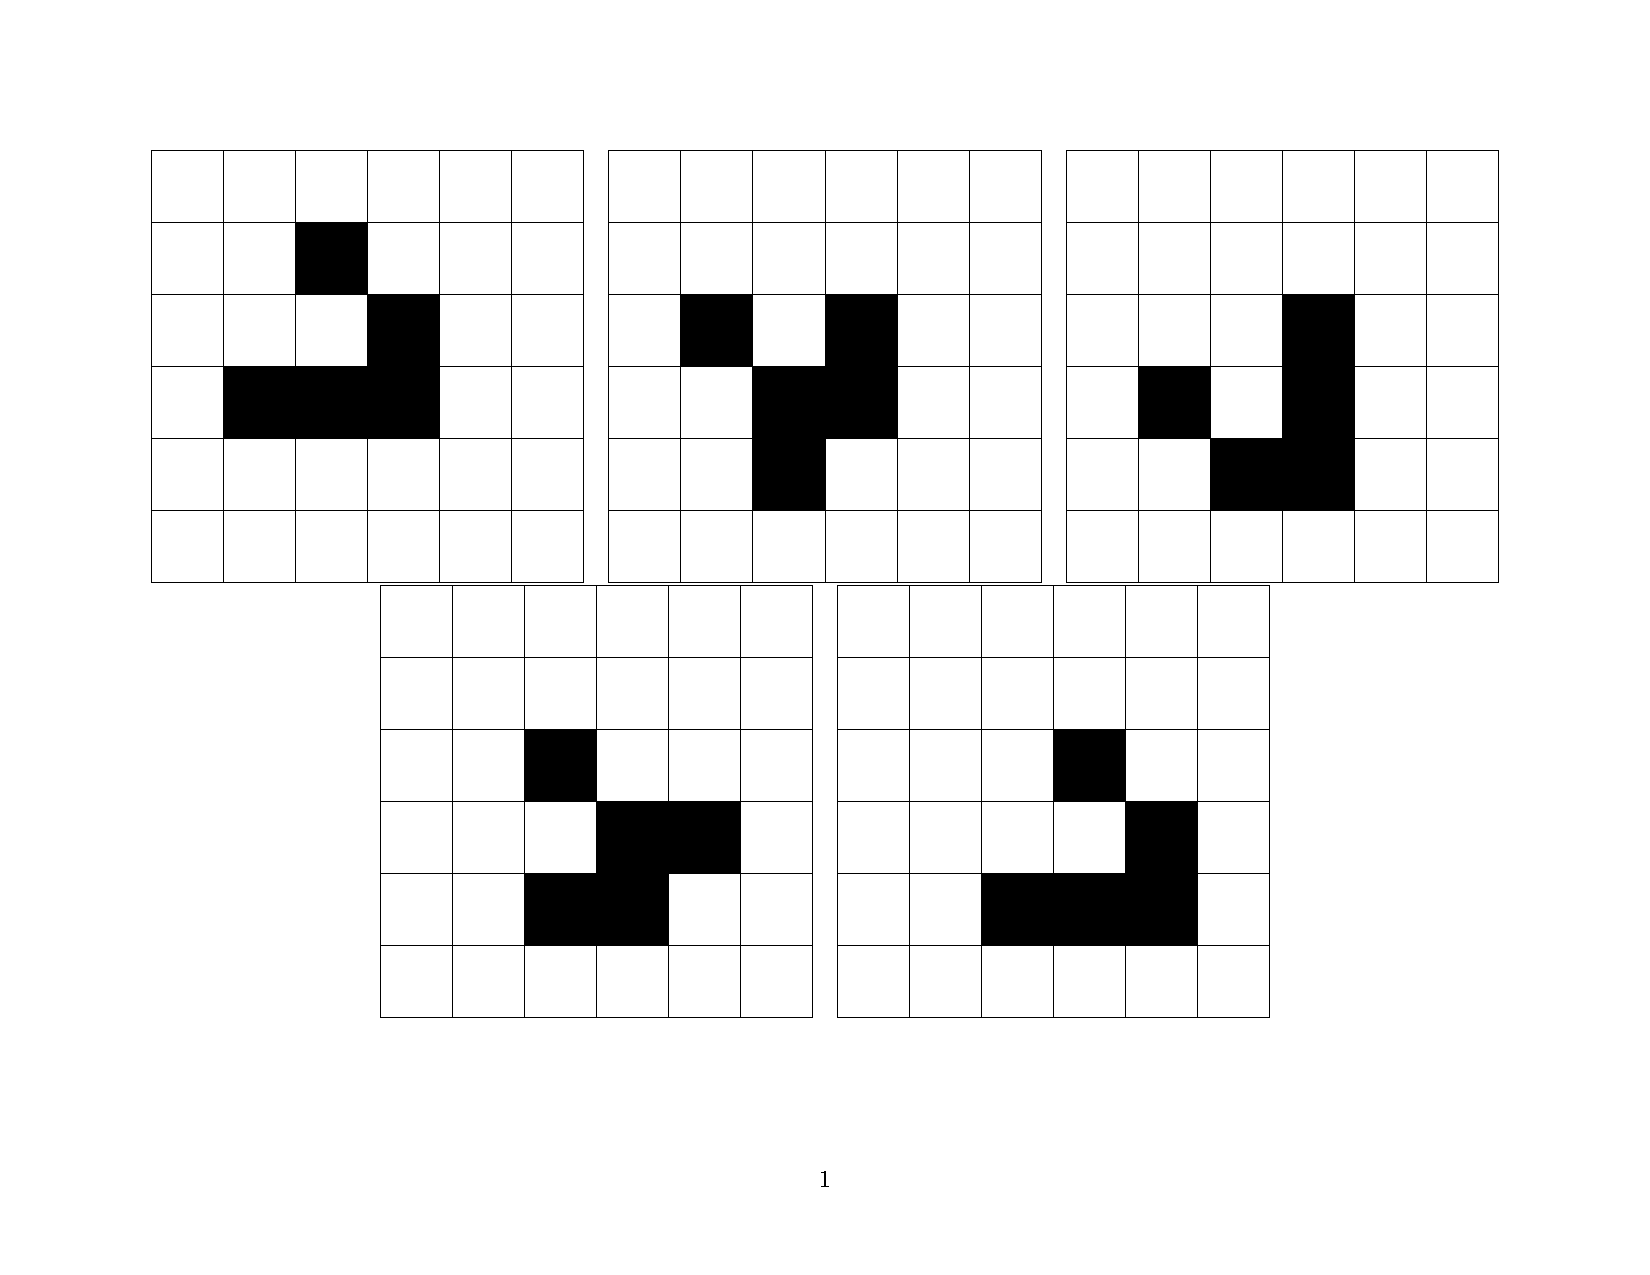
\includegraphics[width=.8\textwidth]{gol_image}
\caption{\label{fig:gol} Un exemple de figure}
\end{figure}

\lipsum[8]

\begin{figure}[tbh]
\centering
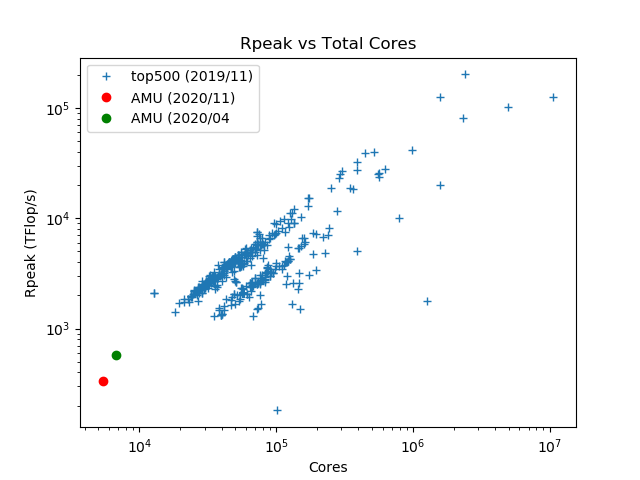
\includegraphics[width=.5\textwidth]{rpeak}
\caption{\label{fig:repeak} Un autreexemple de figure}
\end{figure}

\lipsum[9]

\section{Conclusion}
\lipsum[10]


\bibliographystyle{abbrv}
\bibliography{biblio_projet}

\end{document}